Our cloud path tracing system renders frames for movies in parallel on different virtual machines, as can be seen in Figure~\ref{fig:frame}.

\begin{figure}[ht!]
    \center
    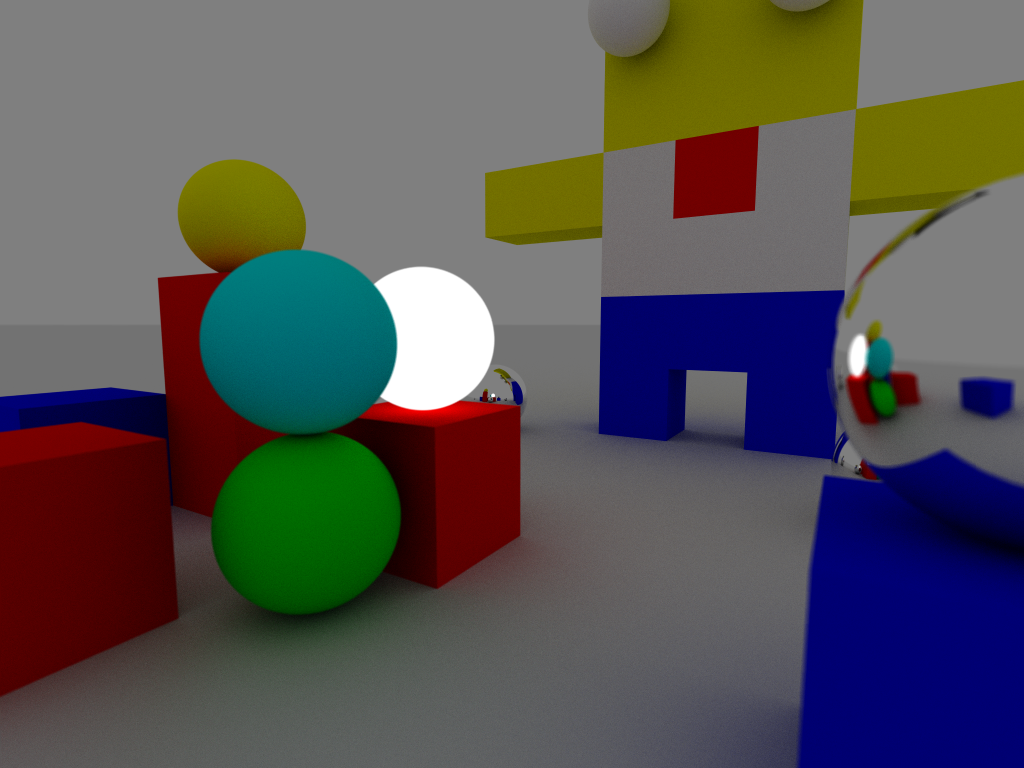
\includegraphics[width=0.45\textwidth]{./img/frame.png}
    \caption{A frame rendered by the cloud path tracer}
    \label{fig:frame}
\end{figure}

From the project description\cite{projectdescription}, the following features were implemented: automation, elasticity, performance, reliability, monitoring and multitenancy.

The system is automated as much as possible, such that the user need only provide the master node with a job description.
All further work is handled by the system itself.

Elasticity is provided in the sense of resource scaling.
When few jobs are running, fewer workers are allocated to do processing.

The experiments show that the load of a job is rather balanced over its workers, leading to good performance.

By making sure that no frames are missing from the end result, even when worker nodes experience unforeseen failure, the system provides reliability.

Using the implemented monitoring features of our system, we have been able to conduct our experiments.

Many different users can tell the system to perform jobs for them at the same time, and thus allows for multitenancy.

For simpler systems, such as web-hosting, there are many SaaS providers that will do a good job without all of the effort.
However, for performance-critical applications such as path tracers, the freedom that IaaS provides allows you to have fine control over the workings of our system as a whole, making it worth the extra effort.